% Editable reader-oriented supplement. Literal examples and scores are generated separately.
\section*{1. Reading the networks}
This supplement adds connected graph views, a temporal explanation and a worked error analysis to the main paper. It is not a second experiment. All outputs, reference answers and assessments are retained from the two reported batches. Codex authored the reference annotations and semantic judgments. These are not independent human review.

\textbf{Two paths.} Pre-extract/select (A) selects existing records from a model extraction made without the question. Contextual extraction (B) independently receives the text and question. A and B graphs are separate outputs, not stages of the same graph.

\textbf{How to read an edge.} Arrows retain subject-to-object direction. Labels show the actual relation (underscores displayed as spaces), citations and any stated bounds or holder/attitude. \texttt{loc} abbreviates \texttt{located\_in}. Identical endpoint strings share a node within a panel. Different strings are never merged for appearance. Parallel assertions remain separate edges. Unprinted qualifiers are null, not timeless truth. A holder badge is a qualification, not an extra model-generated relationship.

\textbf{Assessment and relevance.} + denotes supported meaning, $\sim$ partial meaning, x unsupported and ? unresolved. I denotes supported but irrelevant material. Colour is redundant with labels and line styles. Node fills in Orchard distinguish people, objects and places as display annotations, not inferred ontology types. The broad main-paper extraction is deliberately ungraded rather than presented as a reference graph.

\subsection*{Compact index of retained examples}
\begin{tabular}{L{27mm}L{58mm}L{60mm}}
\toprule
Example & What to inspect & Complete record location\\\midrule
Harbor & Source intervals versus query window (p.~4) & Compact calls 1, 4--6\\
Orchard & Connected ownership slice, extra locations and attribution (pp.~2--3) & Compact calls 2, 7--9\\
Museum & Fresh synthetic comparison, including relevance errors & Compact calls 3, 10--12\\
Fable & Parallel actions, passive wording and conditional scope (pp.~5--6) & Prose calls 1, 4--5\\
Alice & Wrong reading participant and literal thought object (p.~6 and main paper) & Prose calls 2, 6--7\\
Holmes & Syntax failure and unresolved interpretation (pp.~6--7) & Prose calls 3, 8--9\\
\bottomrule
\end{tabular}

Call numbers are local to their batch. Three pre-extractions precede contextual requests in each batch. A pre-extraction reused for several questions is still one model call. The main paper contains the complete aggregate tables. This supplement retains selected explanations instead of repeating every prompt and record. Page~7 gives exact file and field paths for the complete data.

The main Orchard figure is an illustrative selection from an existing evaluation, not a prospectively sampled new success. The views below include extra irrelevant predictions, partial meanings and failures. No record was repaired for display, and no score was recomputed.

\clearpage
\section*{2. Orchard: correct relationships can still be irrelevant}
\textbf{Exact executed ownership/carrying question:} \OrchardQuestion

\begin{center}
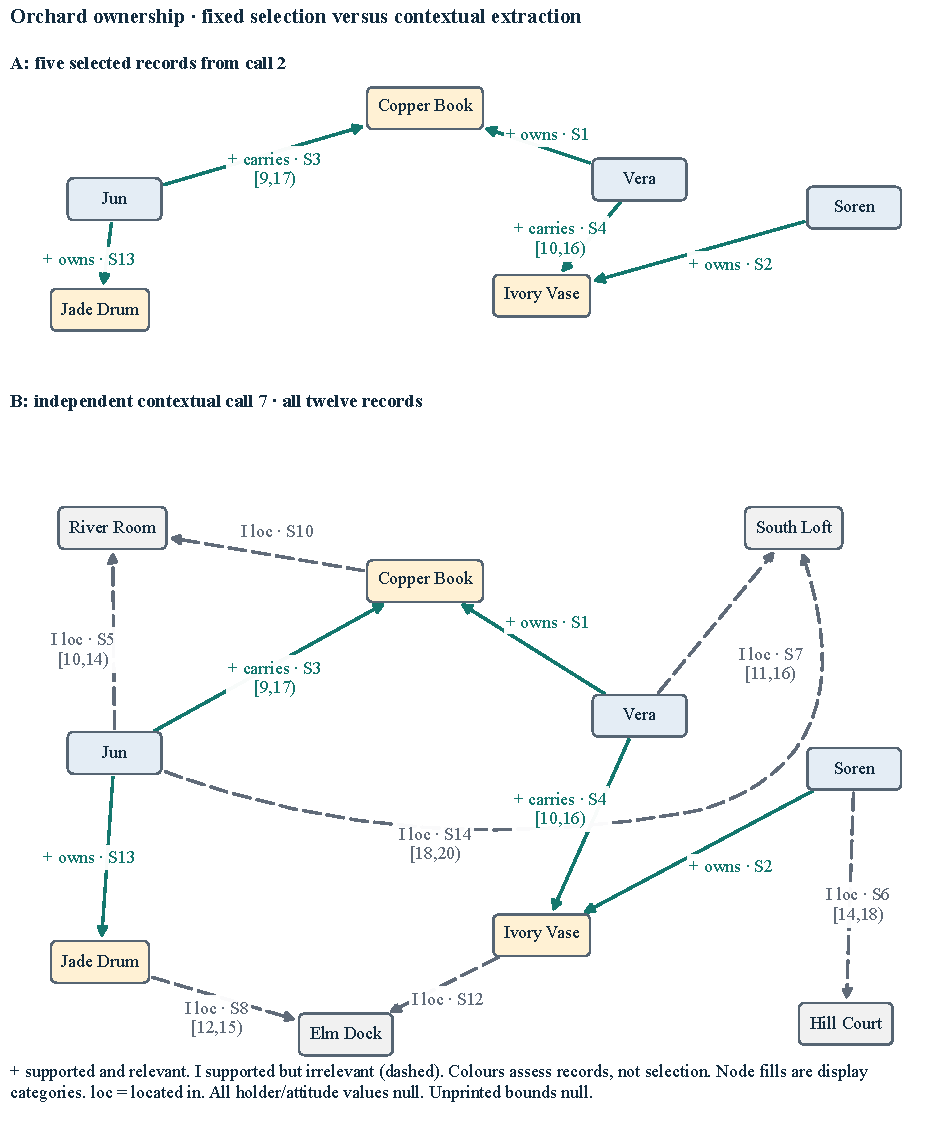
\includegraphics[width=158.0134mm]{figures/orchard_comparison.pdf}
\end{center}
\textbf{A:} \OrchardAScore\quad \textbf{B:} \OrchardBScore

Both views preserve all five requested facts. The contextual output also returns seven locations. These are supported by the supplied story but outside this question. They remain visible and in the precision denominator. No belief records are present in this contextual ownership output. The panels share horizontal anchors and node categories, not an inferred identity mapping across different strings.

\clearpage
\section*{3. Orchard: attribution belongs to the assertion}
\textbf{Exact executed question:} \OrchardBeliefQuestion

\begin{center}
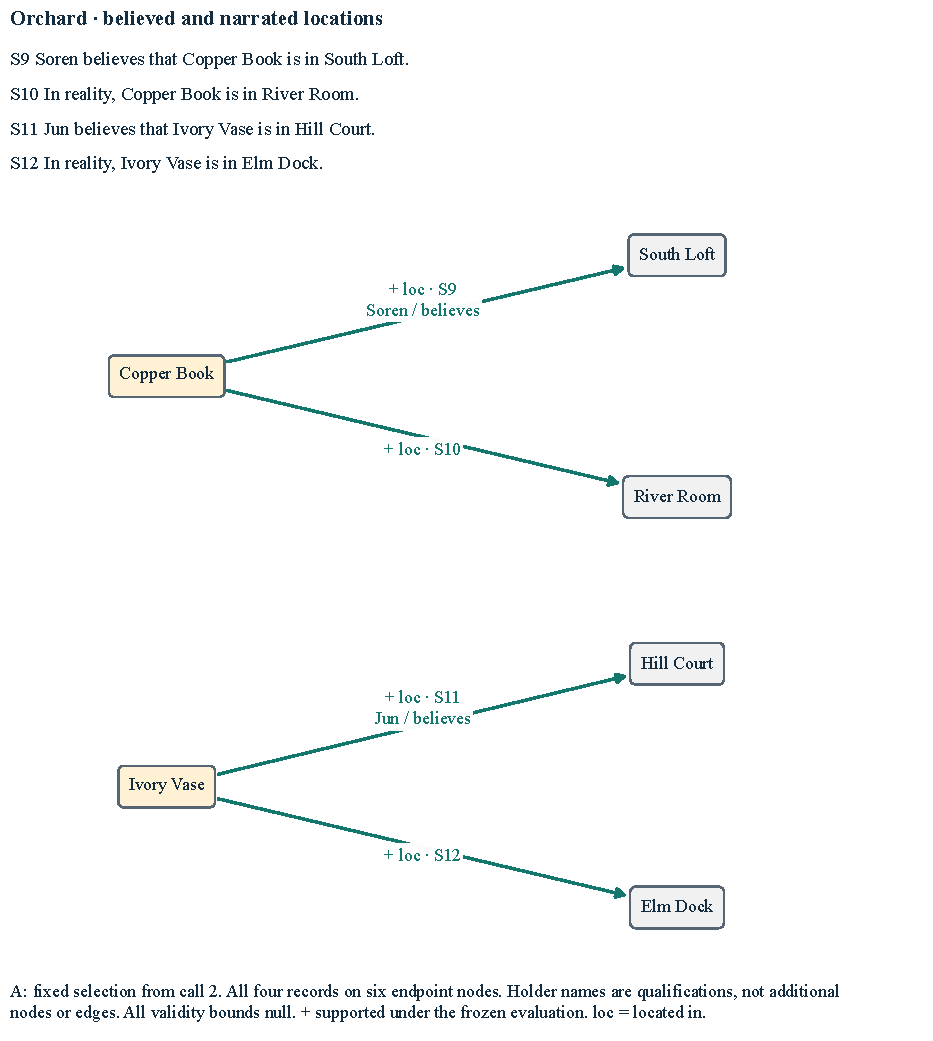
\includegraphics[width=158.0134mm]{figures/orchard_beliefs.pdf}
\end{center}
\textbf{Fixed-selection score:} \OrchardBeliefScore

Each object connects to two places under different epistemic scopes. Copper Book's South Loft location is attributed to Soren's belief, while River Room is narrated reality. Ivory Vase similarly separates Jun's belief from narration. Holder names remain edge metadata even though the names also occur elsewhere in the broader extraction. This selected graph has two disconnected components. No connector has been invented to make it appear more cohesive.

\clearpage
\section*{4. Harbor: preserve source duration, select by overlap}
\textbf{Exact executed question:} \HarborQuestion

\begin{center}
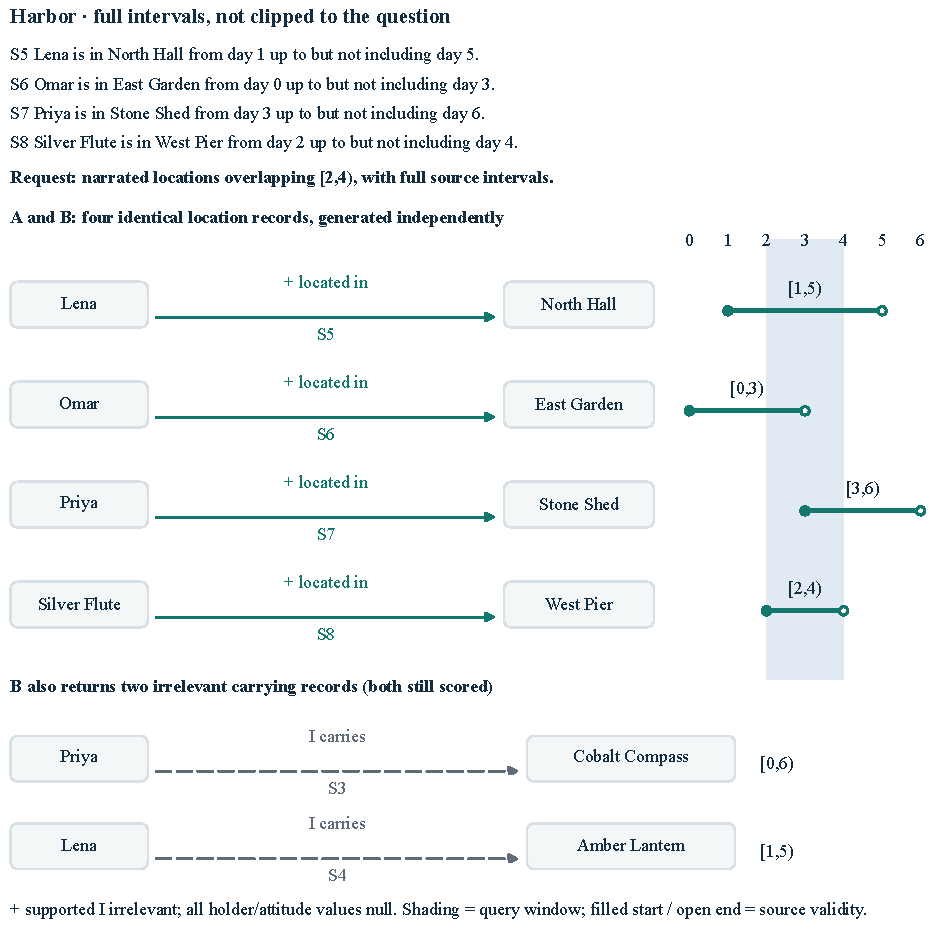
\includegraphics[width=158.0134mm]{figures/harbor.pdf}
\end{center}
The blue band is the requested window $[2,4)$, not rewritten validity. Filled starts and open ends mark the full generated intervals. All four selected A location records coincide with four B records. The two carrying records below are additional B predictions, not part of the location answer. All six B records remain scored. No relationship is given extra temporal precision because it was observed during the question window.

Source display: S5--S8 of the fourteen supplied sentences. Complete evidence and both outputs remain in the compact records. The main paper reports their unchanged strict scores in Table~1.

\clearpage
\section*{5. Fable: parallel actions and separate endpoint identities}
\begin{center}
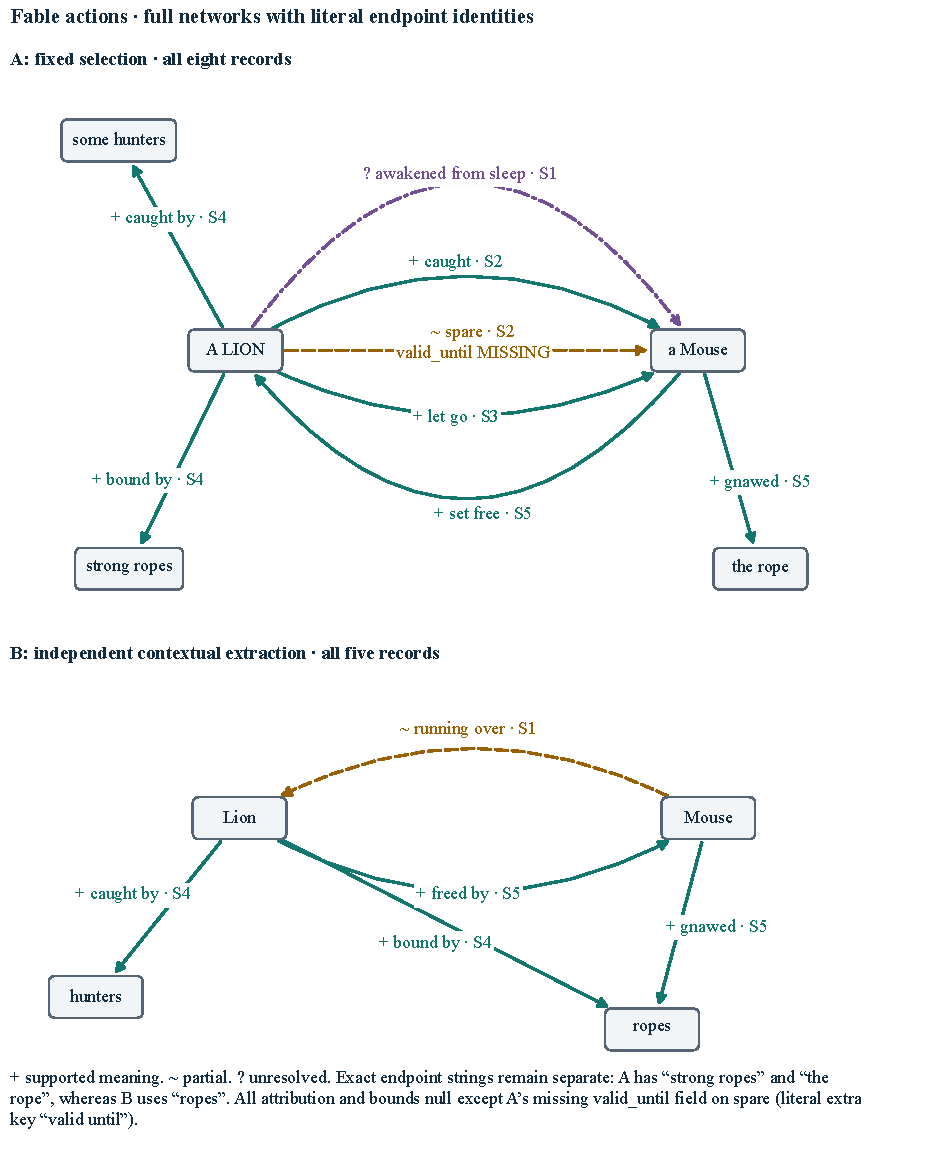
\includegraphics[width=158.0134mm]{figures/fable_networks.pdf}
\end{center}
\textbf{Same executed question as main Figure~2:} \FableQuestion

\textbf{A:} \FableAScore\quad \textbf{B:} \FableBScore

All eight A and five B action records appear. A's five nodes preserve its two different rope strings. B's four nodes use a single literal ropes endpoint. This is not a corrected alias alignment. The complete source is the 133-word fable retained in the prose dataset. A's ambiguous awakening and partial conditional plea remain in the graph.

\clearpage
\section*{6. Agreement, preserved meaning and substantive errors}
\subsection*{A worked example from the fable}
\textbf{Exact supplied S4:} \FableFour

\textbf{Actual contextual record:} \PassiveExample.
Its bounds, holder and attitude are all null. The retained assessment is:
\begin{quote}\PassiveExampleAssessment\end{quote}
The passive relationship preserves the narrated participants and meaning. The frozen strict matcher does not accept that inverse wording. This is a strict mismatch without a semantic falsehood verdict. It is not changed into a matching record for these figures.

\textbf{Exact supplied S1:} \FableOne

\textbf{Actual contextual record:} \PartialExample.
The retained assessment is:
\begin{quote}\PartialExampleAssessment\end{quote}
The broad action survives, but the face-specific endpoint does not. Partial support therefore does not count as complete target coverage. Neither this case nor the passive example is newly scored.

\subsection*{Compact failure and uncertainty guide}
\begin{tabular}{L{29mm}L{54mm}L{62mm}}
\toprule
Issue & Retained example & Interpretation\\\midrule
Wrong participant & Alice contextual actions, record 4: Alice reading the book & Her sister reads. Alice peeps into the book. This is unsupported participant attribution, not merely a synonym mismatch.\\
Belief representation & Alice contextual claims, record 2: literal thought object & Meaning is supported, while the requested decomposed structure is absent. The daisy-chain record remains unresolved.\\
Irrelevant additions & Orchard contextual possession, seven locations & Supported relationships outside the question. Counted as precision errors, not silently removed.\\
Conditional scope & Fable A action record 3: spare & The Mouse's conditional plea is not an unconditional release. The misspelled temporal key also remains.\\
Syntax failure & Holmes pre-extraction and contextual actions & Extra closing brace. No parsed graph scores and no invented empty network.\\
\bottomrule
\end{tabular}

Pending author judgments remain pending, including Holmes's vocative and speaker attribution. Unresolved wording is not assumed true or false.

\clearpage
\section*{7. Reproducibility without repeated data dumps}
\subsection*{Complete records remain available}
Paths below are relative to the conference package unless prefixed by \emph{repository}. They contain the full information that the former 36-page companion printed repeatedly. The data are unchanged.

\begin{tabular}{L{46mm}L{104mm}}
\toprule
File & What to read\\\midrule
\path{data/requests.json} & Exact transmitted payloads, including system and user messages. Select \texttt{compact} or \texttt{prose}, then the string call ID. Request hashes are validated.\\
\path{data/retained_outputs.json} & Complete evidence under \texttt{stories}. Exact raw response strings and parsed records under \texttt{calls}. Full frozen reference alternatives under \texttt{references}. Actual selected/contextual records and evaluations under \texttt{results}.\\
\path{data/evaluation_rules.json} & Frozen normalization, scope and matching rules for each batch.\\
\path{manifest.json} & Exact displayed facts, assessment labels, source call/record mappings, endpoint identities and layout coordinates. Display subsets do not change denominators.\\
\path{generated/reproducibility_index.json} & Hashes and field-level paths connecting this reader guide to complete retained evidence and historical companion version.\\
Repository \path{reports/tables/real_text_proof_of_concept.json} & Complete Codex semantic judgments under \texttt{results[].semantic\_assessments}, plus pre-extraction assessments and syntax diagnoses.\\
Repository \path{reports/tables/compact_story_v2_results.json} & Complete synthetic results, source-support evaluations, selection traces and all historical syntax-recovery categories.\\
\bottomrule
\end{tabular}

The published prose is preserved verbatim with section, edition, retrieval and hash metadata. Project Gutenberg notices remain in \path{data/pg21_notices.txt}, \path{data/pg11_notices.txt} and \path{data/pg1661_notices.txt}. Aesop uses Townsend's translation of \emph{The Lion and the Mouse}; Alice is from Chapter~I, and Holmes from \emph{The Red-Headed League}. Neither familiar context nor later plot information is used to resolve a model record.

\subsection*{A syntax failure is not an empty graph}
\textbf{Holmes contextual actions, retained call 8.} Display excerpt: the final 200 characters, unchanged:
\VerbatimInput[fontsize=\small,breaklines=true,breakanywhere=true]{generated/holmes_tail.txt}
\textbf{Original parser diagnosis:} \HolmesParseError

Only the display is excerpted. The complete raw response remains in \path{data/prose_call_8_raw.txt} and the JSON record. The narrow permitted trailing-comma recovery does not remove an extra closing brace. No graph is reconstructed here.

\subsection*{Provenance and access}
The previous 36-page companion remains in version history. There is one current concise companion. The README gives the portable build and archival retrieval commands. No underlying response, prompt, reference answer or assessment was deleted.

Codex assisted implementation, annotation, assessment and writing. Qwen generated the experimental facts. Human authors retain responsibility, and these semantic judgments are not independent review. Tool citation: OpenAI (2025), \emph{Introducing Codex}, \url{https://openai.com/index/introducing-codex/}. The author checklist records unresolved submission-policy questions.
